\documentclass[12pt, twoside]{article}
\usepackage[letterpaper, margin=1in, headsep=0.2in]{geometry}
\setlength{\headheight}{0.6in}
%\usepackage[english]{babel}
\usepackage[utf8]{inputenc}
\usepackage{microtype}
\usepackage{amsmath}
\usepackage{amssymb}
%\usepackage{amsfonts}
\usepackage{siunitx} %units in math. eg 20\milli\meter
\usepackage{yhmath} % for arcs, overparenth command
\usepackage{tikz} %graphics
\usetikzlibrary{quotes, angles}
\usepackage{graphicx} %consider setting \graphicspath{{images/}}
\usepackage{parskip} %no paragraph indent
\usepackage{enumitem}
\usepackage{multicol}
\usepackage{venndiagram}

\usepackage{fancyhdr}
\pagestyle{fancy}
\fancyhf{}
\renewcommand{\headrulewidth}{0pt} % disable the underline of the header
\raggedbottom
\hfuzz=2mm %suppresses overfull box warnings

\usepackage{hyperref}

\fancyhead[LE]{\thepage}
\fancyhead[RO]{\thepage \\ Name: \hspace{4cm} \,\\}
\fancyhead[LO]{BECA / Dr. Huson / Geometry\\*  Unit 8: Congruence transformations\\* 6 January 2022}

\begin{document}

\subsubsection*{8.4 Classwork: ``Onto'' mappings, symmetry}
\begin{enumerate}
\item What is the smallest non-zero angle of rotation about its center that would map the pentagon onto itself? %$ABCDE$
\begin{center}
    \begin{tikzpicture}[rotate=18, scale=1]
      \draw [thick]
      (0:2)--% node[right] {$A$}--
      (72:2)--% node[above right] {$B$}--
      (144:2)--% node[above left] {$C$} --
      (216:2)--% node[left] {$D$}--
      (288:2)--cycle;% node[right] {$E$}--cycle;
    \end{tikzpicture}
  \end{center}

\item Circle YES or NO to indicate whether the given transformation maps the hexagon onto itself.
\vspace{0.5cm}
\begin{multicols}{2}
 \begin{enumerate}
  \item Yes \quad No \quad A reflection over $\overleftrightarrow{AD}$
  \item Yes \quad No \quad A rotation of $60^\circ$ clockwise around the hexagon's center.
  \item Yes \quad No \quad A reflection over a line through the midpoints of  $\overline{BC}$, $\overline{EF}$.
  \item Yes \quad No \quad A rotation of $120^\circ$ counterclockwise around point $D$.
  \end{enumerate}
\begin{center}
    \begin{tikzpicture}%[scale=.48]
      \draw [thick]
      (0:2)node[right] {$A$}--
      (60:2)node[above right] {$B$}--
      (120:2)node[above left] {$C$} --
      (180:2)node[left] {$D$}--
      (240:2)node[left] {$E$}--
      (300:2)node[right] {$F$}--cycle;
    \end{tikzpicture}
  \end{center}
\end{multicols} \vspace{0.5cm}

\newpage
\item The figure shows a rectangle (not a square).
\begin{center}
  \begin{tikzpicture}[scale=0.7]
    \coordinate (A) at (0, 0); %[label=above left:$P$]
    \coordinate (B) at (4, 0);
    \coordinate (C) at (4, 3);
    \coordinate (D) at (0, 3);
    \draw [thick] (A)--(B)--(C)--(D)--cycle;
    \draw [thick, dashed] (A)--(C);
    \draw [thick] (B)--(D);
    %\draw [thick, xshift=2cm, yshift=2.5cm] (85:3);
  \end{tikzpicture}
\end{center}
Which transformations carries the rectangle onto itself? Mark each True or False.
  \begin{enumerate}
    \item A reflection over the solid diagonal \hfill True \quad False
    \item A reflection over the dashed diagonal \hfill True \quad False
    \item A clockwise rotation of $90^\circ$ about the intersection of the diagonals \hfill True \quad False
    \item A clockwise rotation of $180^\circ$ about the intersection of the diagonals \hfill True \quad False
  \end{enumerate}


\end{enumerate}
\end{document}